
\scsubsection{Введение в описание внешних идентификаторов sc-элементов}
\label{intro_idtf}

\begin{SCn}

\scnsectionheader{\currentname}

\scnstartsubstruct

\scnsegmentheader{Понятие внешнего идентификатора sc-элемента}

\scnstartsubstruct

\scnheader{\currentname}
\scnreltovector{конкатенация сегментов}{Понятие внешнего идентификатора sc-элемента;Понятие простого идентификатора sc-элемента;Понятие сложного идентификатора sc-элемента}

\scnheader{sc-идентификатор}
\scnidtf{внешний идентификатор sc-элемента}
\scntext{пояснение}{Внешние идентификаторы \textit{sc-элементов} (или, сокращенно \scnkeyword{sc-идентификаторы}) необходимы \textit{ostis-системе} исключительно для того, чтобы осуществлять обмен информацией с другими \textit{ostis-системами} или со своими пользователями. Для того чтобы представить свою \textit{базу знаний}, решать самые различные \textit{задачи}, связанные с анализом текущего состояния и эволюцией своей \textit{базы знаний}, задачи, связанные с анализом текущего состояния (текущих ситуаций) окружающей среды, принятием соответствующих решений (целей) и организацией соответствующих \textit{действий}, направленных на выполнение принятых решений (на достижение поставленных целей), \textit{ostis-системе} не нужны никакие внешние идентификаторы (в частности, имена) соответствующие \textit{sc-элементам}. Но для \uline{понимания} сообщений, принимаемых от других субъектов (что для \textit{ostis-системы} означает построение \textit{sc-текста},~~ \textit{семантически эквивалентного} принятому сообщению) и для анализа сообщений, передаваемых другим субъектам (что для \textit{ostis-системы} означает синтез \textit{внешнего текста},~~\textit{семантически эквивалентного} заданному \textit{sc-тексту} и удовлетворяющего некоторым дополнительным требованиям, например, эмоционального характера) \textit{ostis-системе} необходимо знать, как в принимаемом или передаваемом сообщении изображаются (представляются) \textit{знаки}, \uline{синонимичные sc-элементам}, которые уже хранятся или могут храниться в составе \textit{базы знаний}~~\textit{ostis-системы}. В качестве внешних идентификаторов \textit{sc-элементов} чаще всего используются имена (термины) соответствующих (обозначаемых) сущностей, представленные отдельными словами или словосочетаниями на различных естественных языках, но также могут использоваться иероглифы, условные обозначения, пиктограммы.

В общем случае \textit{sc-элементу} может соответствовать несколько синонимичных ему имен на разных \textit{естественных языках}. Более того, \textit{sc-элементу} может соответствовать несколько синонимичных ему имен на одном и том же \textit{естественном языке}. В этом случае одно из этих имен объявляется как основной внешний идентификатор для соответствующего \textit{sc-элемента} и соответствующего \textit{естественного языка}. Основное требование, предъявляемое к таким внешним идентификаторам это отсутствие как синонимов, так и омонимов в рамках множества основных внешних идентификаторов sc-элементов для каждого естественного языка. 

Каждый внешний идентификатор \textit{sc-элемента}, используемый ostis-системой, описывается (представляется) в её памяти в виде \textit{внутреннего файла ostis-системы}, т.е. в виде электронного образа всевозможных вхождений данного внешнего идентификатора во всевозможные внешние тексты соответствующего внешнего языка.}
\scnidtf{внешний идентификатор sc-элемента}
\scnsubdividing{простой sc-идентификатор\\
\scnaddlevel{1}
\scnidtf{простой внешний идентификатор sc-элемента}
\scnaddlevel{-1}
;sc-выражение\\
\scnaddlevel{1}
\scnidtf{сложный внешний идентификатор sc-элемента, в состав которого входит один или несколько идентификаторов других sc-элементов} 
\scnaddlevel{-1}
}
\scnsubdividing{основной sc-идентификатор\\
\scnaddlevel{1}
\scnidtf{основной sc-идентификатор для носителей дополнительно указываемого языка общения (например, соответствующего естественного языка)}
\scnsuperset{основной международный sc-идентификатор}
\scnaddlevel{1}
\scntext{примечание}{В качестве \textit{основных sc-идентификаторов} могут использоваться также общепринятые международные условные обозначения некоторых сущностей, например, обозначения часто используемых функций (sin, cos, tg, log, и т.д.), единиц измерения, денежных единиц и многое другое. Формально каждый основной международный sc-идентификатор считается основным sc-идентификатором также и для каждого естественного языка, несмотря на то, что символы, используемые в основных международных sc-идентификаторах, могут не соответствовать алфавиту некоторых или даже всех естественных языков.}
\scnaddlevel{-1}
\scnsuperset{системный sc-идентификатор}
\scnaddlevel{1}
\scnidtf{основной sc-идентификатор для языка общения между ostis-системами}
\scnaddlevel{1}
\scntext{примечание}{В качестве указанного языка общения между ostis-системами используется SCs-код.}
\scnaddlevel{-1}
\scntext{примечание}{системный sc-идентификатор часто совпадает с основным англоязычным sc-идентификатором.}
\scnaddlevel{-2}
;неосновной sc-идентификатор\\
\scnaddlevel{1}
\scntext{примечание}{С помощью неосновных sc-идентификаторов указываются возможные \textit{синонимы*} соответствующего \textit{основного sc-идентификатора}, которые в частности, могут пояснять или даже определять обозначаемую сущность, указывает на важные свойства этой сущности.}
\scnsuperset{{\normalfont(}неосновной sc-идентификатор $\cap$ пояснение{\normalfont)}}
\scnaddlevel{1}
\scnidtf{неосновной sc-идентификатор, являющийся одновременно и пояснением обозначаемой сущности}
\scnsuperset{{\normalfont(}неосновной sc-идентификатор $\cap$ определение{\normalfont)}}
\scnaddlevel{1}
\scnidtf{неосновной sc-идентификатор, являющийся одновременно и определением обозначаемого понятия}
\scnaddlevel{-2}
\scnsuperset{неосновной часто используемый sc-идентификатор}
\scnaddlevel{1}
\scntext{пояснение}{Для некоторых sc-элементов могут часто использоваться не только основные, но и неосновные sc-идентификаторы (особенно в неформальных текстах -- в пояснениях, примечаниях и т.п.). Явное выделение такого класса sc-идентификаторов позволяет упростить семантический анализ исходных текстов баз знаний.}
\scnaddlevel{-2}
}
\scntext{примечание}{Каждому sc-элементу может соответствовать целое семейство внешних идентификаторов этого sc-элемента, которые обычно являются терминами, именующими обозначаемую сущность. Среди этих внешних идентификаторов для каждого идентифицируемого sc-элемента выделяется один как основной идентификатор. А неосновные термины (имена), соответствующие этим sc-элементам (в том числе и sc-классам), поясняют денотационную семантику указанного sc-элемента.}

\bigskip
\scnstartset
\scnheader{основной sc-идентификатор}
\scnsubset{файл-образец ostis-системы}
\scnendstruct

\scnrelboth{семантическая эквивалентность}{\scnfilelong{Все основные идентификаторы sc-элементов в памяти ostis-системы оформляются в виде копируемых фалов-образцов ostis-системы.}}
\scnaddlevel{1}
\scntext{пояснение}{Копии основных sc-идентификаторов входят в состав внешних текстов различных языков (SCg-кода, SCs-кода, SCn-кода), а также в различных падежах, склонения, спряжениях в состав файлов ostis-систем.}
\scnaddlevel{-1}
\scntext{примечание}{Аналогичное утверждение справедливо и для неосновных часто используемых sc-идентификаторов. Все остальные неосновные sc-идентификаторы считаются вспомогательными файлами-экземплярами.}

\scnheader{sc-идентификатор}
\scnsubdividing{строковый sc-идентификатор\\
\scnaddlevel{1}
\scnidtf{sc-идентификатор, представленный строкой символов, которая является именем обозначаемой сущности}
\scnidtf{имя сущности, обозначаемой идентифицируемым sc-элементом}
\scnidtf{имя (термин, словосочетание), синонимичное соответствующему (идентифицируемому) sc-элементу и представленное в соответствующем алфавите символов}
\scnaddlevel{-1}
;sc-идентификатор, представленный иероглифами;sc-идентификатор, представленный условным обозначением или пиктограммой}
\scntext{примечание}{Введенные нами sc-идентификаторы используются во всех внешних языках, близких SC-коду -- в SCg-коде, в SCs-коде и в SCn-коде.}

\scnheader{строковый sc-идентификатор}
\scnidtf{имя, приписываемое идентифицируемому sc-элементу}
\scnidtf{имя сущности, обозначаемой идентифицируемым sc-элементом}
\scnidtf{строка символов, синонимичная соответствующему идентифицируемому sc-элементу}
\scnsuperset{основной строковый sc-идентификатор}
\scnaddlevel{1}
\scnidtf{уникальное для каждого естественного языка внешнее имя, приписываемое идентифицируемому sc-элементу}
\scnsuperset{основной русскоязычный sc-идентификатор}
\scnsuperset{системный sc-идентификатор}
\scnsuperset{основной англоязычный sc-идентификатор}
\scnsuperset{основной германоязычный sc-идентификатор}
\scnsuperset{основной франкоязычный sc-идентификатор}
\scnsuperset{основной италоязычный sc-идентификатор}
\scnsuperset{основной китайскоязычный sc-идентификатор}
\scnaddlevel{-1}
\scnheader{sc-идентификатор}
\scntext{примечание}{Представление знаков в виде неатомарных фрагментов информационных конструкций (в частности, в виде имен обозначаемых сущностей, построенных в фиксированном алфавите), взаимно однозначно соответствующих обозначенным сущностям, необходимо только для того, чтобы иметь простую процедуру установления синонимии знаков, входящих в состав одной или разных информационных конструкций.}

\scnendstruct

\scnsegmentheader{Понятие простого идентификатора sc-элемента}

\scnstartsubstruct

\scnheader{простой идентификатор sc-элемента}
\scntext{правила построения}{Правила построения простых sc-идентификаторов.\\
Данные правила включают в себя:
\begin{scnitemize}
    \item Символы, используемые в простых sc-идентификаторах (в том числе, специальные символы);
    \item Специальные предикаты, используемые в простых sc-идентификаторах;
    \item Специальные суффиксы, используемые в простых sc-идентификаторах;
    \item Разделители, используемые в простых sc-идентификаторах;
    \item Ограничители, используемые в простых sc-идентификаторах;
    \item Правила построения простых sc-идентификаторов, определяемые различными классами идентифицируемых сущностей;
    \item Правила построения sc-имен собственных и sc-имен нарицательных.
\end{scnitemize}
Общим правилом построения простых sc-идентификаторов является стремление максимально возможным образом использовать сложившуюся терминологию. Но при этом следует подчеркнуть, что необходимость исключения омонимии в sc-идентификаторах требует строгого формального \uline{уточнения} семантической интерпретации каждого используемого термина. Особо подчеркнем то, что в ostis-системах процесс построения новых терминов (sc-идентификаторов) и процесс совершенствования существующей терминологии по отношению к процессу развития ostis-систем, баз знаний, представленных в SC-коде, с технической точки зрения абсолютно не зависят друг от друга. Кроме того, следует помнить, что \uline{далеко не все} sc-элементы, входящие в состав базы знаний ostis-системы, должны иметь соответствующие им sc-идентификаторы (быть идентифицированными). Очевидно, что идентифицированными (именованными) должны быть все используемые понятия, вводимые в соответствующих предметных областях и специфицируемые соответствующими онтологиями. Идентифицированными также должны быть обладающие особыми свойствами ключевые экземпляры (элементы) некоторых понятий, различные социально значимые объекты (персоны, населенные пункты, географические объекты, страны, организации, библиографические источники и многое другое).\\
Рассмотрим правила построений простых sc-идентификаторов, определеяемые различными классами идентифицируемых сущностей:
\begin{scnitemize}
    \item Первым символом каждого простого sc-идентификатора и каждого сложного sc-идентификатора, идентифицирующего sc-переменную (переменный sc-элемент), является подчеркнутый пробел;
    \item Последним символом простого sc-идентификатора, идентифицирующего sc-узел, обозначающий неролевое отношение, заданное на множестве sc-элементов, является крестик в виде верхнего индекса;
    \item Последним символом простого sc-идентификатора, идентифицирующего sc-узел, обозначающий заданное на множестве sc-элементов ролевое отношение (т.е. отношение, являющееся подмножеством отношения принадлежности), является апостроф (черточка в виде верхнего индекса);
    \item Последним символом простого sc-идентификатора, идентифицирующего sc-узел, обозначающий понятие, не являющееся отношением, (таковыми, в частности, являются различного рода параметры — длина, площадь, объем, масса) является звездочка в виде верхнего индекса;
    \item В рамках SCs-кода целесообразно вводить правила унифицированного построения простых sc-идентификаторов и целого ряда других классов идентифицируемых сущностей — персон, библиографических источников (публикаций), разделов баз знаний ostis-систем, файлов ostis-систем, самих ostis-систем.
\end{scnitemize}}

\scnheader{имя нарицательное}
\scnidtf{имя, которое может быть приписано \uline{любому} экземпляру некоторого класса и которое обозначает указанный класс}
\scntext{примеры}{треугольник; город; персона; отношение; параметр; константа; переменная}
\scnnote{\textit{имя нарицательное} всегда начинается с маленькой буквы}

\scnheader{имя собственное}
\scnidtf{имя, которое либо не является обозначением какого-либо класса сущностей, либо является обозначением (именем) некоторого класса сущностей, но построенным без использования нарицательного имени этого класса, либо является именем некоторого класса сущностей, построенным с использованием нарицательного имени этого класса (1) путем преобразования имени нарицательного во множественное число или (2) путем дополнительного использования в начале формируемого имени собственнного таких терминов, как "Класс...", "Множество...", "Множество всевозможных...".}
\scntext{примеры}{Москва; Иванов Иван Сергеевич; Точка А; Город Минск; SC-код; Русский язык; Множество всевозможных sc-текстов; Класс sc-текстов; Класс русскоязычных текстов.}
\scnnote{имя собственное всегда начинается с большой буквы}

\scnendstruct

\scnsegmentheader{Понятие сложного идентификатора sc-элемента}

\scnstartsubstruct

\scnheader{сложный sc-идентификатор}
\scnsuperset{сложный sc-идентификатор, идентифицирующее sc-коннектор}
\scnsuperset{сложный sc-идентификатор, ограничиваемое фигурными скобками и обозначающее множество sc-элементов, все sc-идентификаторы которых перечисляются}
\scnsuperset{сложный sc-идентификатор, ограничиваемое фигурными скобками и обозначающее множество sc-элементов, входящих в состав sc-текста, который семантически эквивалентен тому тексту (sc.s-тексту, sc.g-тексту, ея-тексту и т.д.), который ограничен указанными фигурными скобками}
\scnsuperset{сложный sc-идентификатор, ограничиваемое квадратными скобками и обозначающее файл-экземпляр ostis-системы}
    \scnaddlevel{1}
    \scnrelfrom{смотрите}{Принципы SC-кода}
        \scnaddlevel{1}
        \scniselement{секция раздела базы знаний}
        \scnaddlevel{-1}
    \scnaddlevel{-1}
\scnsuperset{сложный sc-идентификатор, ограничиваемое квадратными скобками и дополнительными вертикальными линиями (или кавычками) и обозначающее файл-класс ostis-системы}
    \scnaddlevel{1}
    \scnrelfrom{смотрите}{Принципы SC-кода}
        \scnaddlevel{1}
        \scniselement{секция раздела базы знаний}
        \scnaddlevel{-1}
    \scnaddlevel{-1}
\scnsuperset{сложный sc-идентификатор, использующее знаки алгебраических операций}
    \scnaddlevel{1}
    \scntext{примеры}{($s_i \cup s_j \cup s_k$); ($s_i \cap s_j \cap s_k$); ($s_i \backslash s_j$); ($x+y+z$); ($x \times y \times z$)}
    \scnaddlevel{-1}
\scnsuperset{сложный sc-идентификатор, обозначающее второй компонент пары указываемого ориентированного бинарного или квазибинарного отношения для указываемых аргументов\\
    \scnaddlevel{1}
    \scntext{примеры}{объединение*($s_i$; $s_j$; $s_k$); пересечение*($s_i$; $s_j$; $s_k$); разность множеств*($s_i$; $s_j$); сложение*($x$; $y$; $z$); умножение*($x$; $y$; $z$); sin*($x$); cos*($x$)}
    \scnaddlevel{-1}}
\scnexplanation{Использование сложныйх sc-идентификаторов позволяет существенно сократить число "придумываемых"\ sc-идентификаторов, каковыми в конечном счете становятся только простые sc-идентификаторы, поскольку, зная то, как связан идентифицируемый sc-элемент с теми sc-элементами, которые уже имеют sc-идентификаторы, во многих случаях можно построить сложный sc-идентификатор, идентифицирующее указанный sc-элемент. Кроме того, каждое сложный sc-идентификатор, являясь внешним идентификатором, является также и \uline{транслируемым} формальным текстом, содержащим некоторую информацию об обозначаемой ею сущности.}

\scnheader{сложный sc-идентификатор, идентифицирующий sc-коннектор}
\scnnote{Поскольку кратные sc-коннекторы одного и того же вида встречаются редко, сложный sc-идентификатор, идентифицирующий sc-коннектор, чаще всего \uline{однозначно} идентифицирует соответствующий sc-коннектор. В случае кратных sc-коннекторов одинакового семантического вида, отражаемого типом sc.s-коннектора, можно, например, sc-идентификаторам, идентифицирующим разные кратные sc-коннекторы, приписывать разные номера. Пусть, например, sc-элементы $e_i$ и $e_j$ соединены двумя \uline{кратными} константными постоянными sc-дугами. Тогда указанные sc-дуги можно идентифицировать следующими sc-идентификаторами:\\
($e_i => e_j$)1\\
($e_i => e_i$)2\\}

\scnheader{Файл-рисунок на странице 125}
\scnexplanation{В данном файле ostis-системы приведено определение понятия сложный sc-идентификатор, идентифицирующий sc-коннектор, представленное в SCg-коде и на Языке Бэкуса-Наура.}

\scnheader{Таблица.Типология сложных sc-идентифкаторов}
\scneqfile{\\
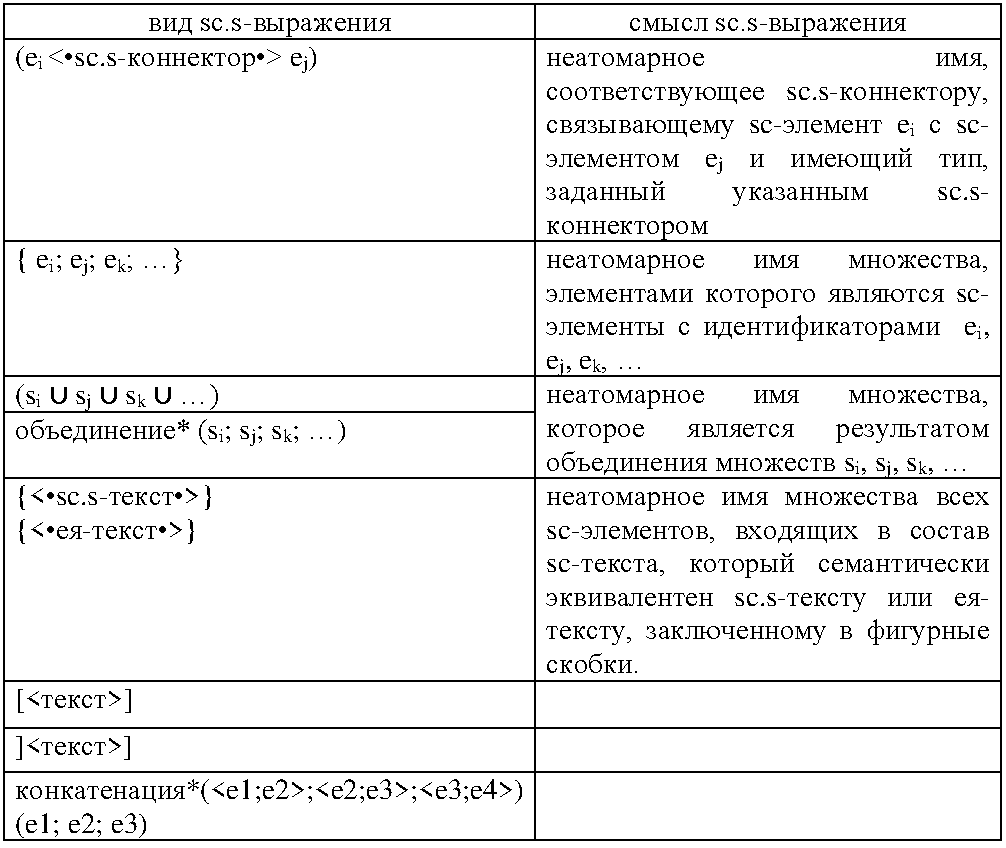
\includegraphics[width=1\linewidth]{figures/intro/scs-statements.pdf}\\
}

\scnendstruct \scninlinesourcecommentpar{Завершили представление Сегмента "\textit{Понятие сложного идентификатора sc-элемента}"}

\scnendstruct \scninlinesourcecommentpar{Завершили \textit{Введение в описание внешних идентификаторов sc-элементов}}

\end{SCn}
    